\chapter{Review of production mechanism and experimental status}
\label{sec:review}
\chaptermark{Review}
The Standard Model (SM) is the theory which describes the electromagnetic, weak
and strong interactions between elementary particles. The model describes a
wide variety of subatomic phenomena involving known elementary particles and
has been confirmed with high precision measurements. This theory is based on
the quark model started in the 1960s\cite{GellMann:1964nj,Zweig:1981pd}, few
years before the experimental confirmation of the existence of quarks. The
theory says that quarks are elementary particles which interact due to the
strong interaction. Because of a phenomenon called color confinement, they are
never been directly observed,  but can be found within composite particles
called hadron. There are two types of hadrons named as baryons (qqq), made of
three quarks or anti-quarks, and mesons ($q\bar{q}$), made of one quark and
anti-quark. The quark model is composed of 6 different types of quarks known as
flavors: up (u), down (d), strange (s), charm (c), bottom or beauty (b), top or
truth (t).

Quarkonia, i.e. the bound states of heavy quark-antiquark pairs, are
particularly interesting in this context, since they provide a testing ground
of QCD in a relatively simple and calculable environment. Also, production of
quarkonia at LHC represents an interesting check of production mechanisms and
models. Toponia ($t\bar{t}$) states are expected to decay very quickly, due to
the heavy top quark mass, and have never been observed. The experimentally
established quarkonia consist therefore of charmonium ($c\bar{c}$) and
bottomonium ($b\bar{b}$) states.

The $\jpsi$ meson, made up of $c\bar{c}$, was the first observed quarkonium
state\cite{PhysRevLett.33.1404}, with a mass around 3.1\gev and narrow width. The analogous 
bound state in the $b$ sector was established with the observation of the 
$\Upsilon(1S)$ meson in 1977 \cite{Herb:1977ek}. 
There is a wide variety of quarkonium states, each differing from other by quantum
numbers: the principal quantum number ($n$), the relative angular momentum
between the quarks ($L$), the spin combination of the two quarks ($S$) and the total
angular momentum ($J$) with $J = L + S$. In particle physics, the notation $J^{PC}$ is
often used, where $P$ is the parity number and $C$ is the charge conjugation number.
For the quarkonium states, they are defined as $P=(-)^{L+1}$ and $C=(-)^{L+S}$.
Table \ref{tab:quarkonium} shows the properties of the quarkonium states. 

\begin{table}[H]
\centering
\caption{Properties of quarkonium states relevant in this thesis.}
% \resizebox{.75\textwidth}{!}{
\begin{tabular}{lccl}\toprule
Meson & $n^{2S+1} L_J$ &  $J^{PC}$ & Mass (\mevcc)\\
\midrule
$\eta_c(1S)$    & $1^1 S_0$ & $0^{-+}$ & $2980.4 \pm 1.2$ \\
$\jpsi(1S)$    & $1^3 S_1$ & $1^{--}$ & $3096.916 \pm 0.011$ \\
$\chi_{c0}(1P)$ & $1^3 P_0$ & $0^{++}$ & $3414.75 \pm 0.31$ \\
$\chi_{c1}(1P)$ & $1^3 P_1$ & $1^{++}$ & $3510.66 \pm 0.07$ \\
$h_{c}(1P)$     & $1^3 P_1$ & $1^{++}$ & $3525.93 \pm 0.27$ \\
$\chi_{c2}(1P)$ & $1^3 P_2$ & $2^{++}$ & $3556.20 \pm 0.09$ \\
$\eta_{c}(2S)$  & $2^1 S_0$ & $0^{-+}$ & $3637 \pm 4$ \\
$\psi(2S)$      & $2^3 S_1$ & $1^{--}$ & $3686.09 \pm 0.04$ \\
\midrule
$\eta_b$        & $1^1 S_0$ & $0^{-+}$ & $9388.9 \pm 2.5 \pm 2.7$ \\
$\Upsilon(1S)$  & $1^3 S_1$ & $1^{--}$ & $9460.30 \pm 0.26$\\
$\chi_{b0}(1P)$ & $1^3 P_0$ & $0^{++}$ & $9859.44 \pm 0.42 \pm 0.31$ \\
$\chi_{b1}(1P)$ & $1^3 P_1$ & $1^{++}$ & $9892.78 \pm 0.26 \pm 0.31$ \\
$\chi_{b2}(1P)$ & $1^3 P_2$ & $2^{++}$ & $9912.21 \pm 0.26 \pm 0.31$ \\
$\Upsilon(2S)$  & $2^3 S_1$ & $1^{--}$ & $10023.26 \pm 0.31$ \\
$\chi_{b0}(2P)$ & $2^3 P_0$ & $0^{++}$ & $10232.5 \pm 0.4 \pm 0.5$ \\ 
$\chi_{b1}(2P)$ & $2^3 P_1$ & $1^{++}$ & $10255.46 \pm 0.22 \pm 0.5$ \\ 
$\chi_{b2}(2P)$ & $2^3 P_2$ & $2^{++}$ & $10268.65 \pm 0.22 \pm 0.5$ \\ 
$\Upsilon(3S)$  & $2^3 S_1$ & $1^{--}$ & $10355.2 \pm 0.5$ \\
\bottomrule
\end{tabular}
% }
\label{tab:quarkonium}
\end{table}

\begin{figure}[H]
  \setlength{\unitlength}{1mm}
  \centering
  \resizebox{\textwidth}{!}{
  \begin{picture}(150,80)
  \put(0,0){\includegraphics*[width=150mm, height=80mm]{bottomonium}}
  \put(3,25){\Large \begin{sideways}$m(b\bar{b}) \left[\gevcc\right]$\end{sideways}}
  \end{picture}
  }
\caption{Observed (blue) and theoretically predicted (red) bottomonium states}
\label{fig:bottomonium}
\end{figure} 



All bottomonium states and their quantum numbers are shown
in~\Cref{fig:bottomonium}. The $L = 0$ and $L = 1$ states are respectively
called S-wave and P-wave. For example, \Y1S is a S-wave and \chiboneOneP is a
P-wave. The principal quantum number $n$ orders states from lowest to highest
masses, such as for $\Upsilon(nS)$, where $n$ equals to 1, 2, 3 and 4. When the
conditions $L = 1$ and $S = 1$ are satisfied, J takes the value 0, 1 or 2
causing mass level splitting, which is called the spin-orbit coupling. Thus,
each \chib states has three sub-states indexed by the value of the quantum
number J. For example, $\chi_b(1P)$ state has three sub-states $\chi_{bJ}(1P)$,
where n equals to 1, 2 and 3.

Radiative transition from one bottomonium state to another is possible to
observe. This transition involve a photon in the final state. The selection
rules are the same as for the hydrogen atom energy states. The electric dipole
transition is the leading order transition, which changes the relative angular
momentum $\Delta L  = \pm 1$ but not the spin $\Delta S = 0$. The magnetic
dipole transition is a next to leading order transition and therefore is very
rare. This transition changes the spin $\Delta S = \pm 1$ but not the relative
angular momentum $\Delta L = 0$.

\section{The quarkonium mass spectrum}

Many theoretical models have been developed to describe quarkonium systems.
These models can be roughly split in two classes, based respectively on Lattice
QCD calculations and phenomenological approaches. The simplest and most
frequently used phenomenological approach is the {\it non-relativistic
potential model}, an effective theory in which the quark move non-
relativistically inside hadrons. Similarly to the positronium case, the system
involves a typical velocity $v$ given by the strong coupling constant
$\alpha_s$, evaluated at a scale corresponding to the typical size of the bound
state

\begin{equation}
v \approx \alpha_s(1/r^2), r \approx 1/mv
\end{equation}

\noindent Being $v$ larger than $\alpha_s(m^2)$, higher-order corrections to the 
non-relativistic approximation are potentially more important than higher-order
perturbative corrections. So far the theoretical calculations of charmonium and
bottomonium and their spectra measured by many experiments suggest that the
potential of quarkonium possesses a radial dependence of an approximately
Coulomb form at small distances due to gluon exchange

\begin{equation}
V(r) \approx -{\frac{4}{3}}{\frac{\alpha_s(1/r^2)}{r}} \quad (r\rightarrow 0)
\end{equation}
\noindent and is confining at large distances due to the increasing strength 
of the coupling
\begin{equation}
V(r) \approx kr \quad (r\rightarrow \infty)
\end{equation}

\noindent where k is the string tension and the factor of 4/3 arises from the
SU(3) colour factors. Several models have been widely used for explaining the
quarkonium spectroscopy. Although these potentials have different asymptotic
behaviours at small and large distances, they coincide with each other in the
region $0.1 fm < r <1 fm$, where $r$ is the average distances between heavy quarks
in the bound systems. Experimental measurements can be used as inputs to
understand the exact shape of the strong potential. For instance, the Cornell
model

\begin{equation}
V_C(r) = -{\frac{4}{3}}{\frac{\alpha_s}{r}} + {\frac{r}{a^2}} + c_0
\end{equation}  

\noindent describes the fine and hyperfine structures of charmonium levels in the leading
non-relativistic treatment. By using charmonium data, the coefficients are
determined to be $\alpha_s = 0.36$, $a=2.34 \gev^{-1}$, $c_0 = -0.25 \gev$, $m_c
= 1.84\gev$.

Energy levels and wave functions of the quarkonium system are obtained by solving 
the non-relativistic Schr\"odinger equation in terms of the constituent masses and the 
potential function. The wavefunction, $\Psi(r) = \Psi_{nL}(r)Y_{Lm}(\theta,\phi)$, with 
$\Psi_{nL}(r)$ and $Y_{Lm}(\theta,\phi)$ being the radial and orbital parts of the wavefunction, 
gives predictions of quarkonium properties. The radial wavefunctions of the $\jpsi$ and 
$\psi(2S)$ systems from various potential models are shown in \Cref{fig:psipot}. 
Up to 30\% differences can be noticed at small values of $r$. 

\begin{figure}
\center
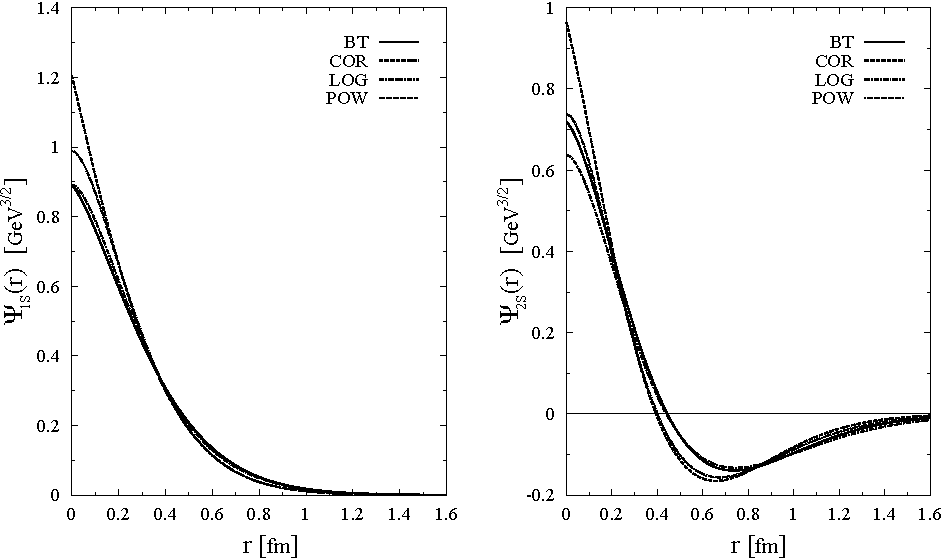
\includegraphics[width=\textwidth]{figs/review/psipot}
\caption{Radial Wave functions for the $\jpsi$ (left) and $\psi(2S)$ (right) for different 
potential models: Buchm\"uller and Tye (BT), Cornell (COR), Logarihmic (LOG) and Power (POW). }
\label{fig:psipot} 
\end{figure} 


\section{Quarkonium production}

The production of quarkonium states can be split in two parts: the production
of a heavy quark-antiquark pair in the regime of perturbative QCD, and the
formation of a bound state, which is driven by non-perturbative QCD. Many
theoretical models have been proposed to interpret the quarkonium production
rates measured by experiments.

\subsection{Colour Singlet Model}

\begin{figure}
\center
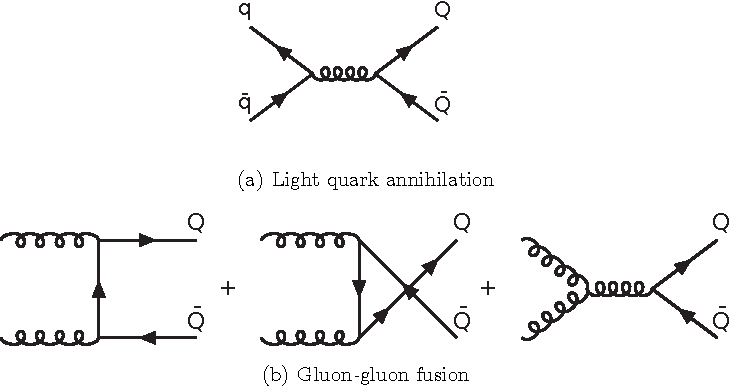
\includegraphics[width=\textwidth]{figs/review/heavy}
\caption{Leading-order Feynman diagrams for heavy quark production\cite{Ellis:318585}}
\label{fig:heavy} 
\end{figure} 


The leading order diagrams for the production of a $Q\bar{Q}$ pair are shown in
\Cref{fig:heavy}. Quark-antiquark annihilation produces a pair in an octet
state, while gluon-gluon fusion can give a  pair in either a singlet or an
octet state, mainly the latter. The Colour Singlet Model (CSM)\cite{Humpert:171969}
assumes that a given quarkonium state can only be produced from a heavy quark
pair with the same quantum numbers. In particular, the the quark pair must have
the same spin and colour state as the final quarkonium state, i.e. colour
neutral. The formation of a quarkonium bound state is parameterised by
non-perturbative theory in the CSM into one single term, assuming the constituent
quarks are at rest in the meson frame ({\it{static approximation}}). The 
short-distance cross section for the whole process can be written as

\begin{equation}
d{\hat{\sigma}}(ij\rightarrow H + X) = d{\hat{\sigma}}(ij\rightarrow Q{\bar{Q}}\left[n^{2S+1}L_J\right] + X) 
|\Psi^{(k)}_{nL}(0)|^2
\end{equation}

\noindent where the radial wave functions at the origin can be extracted from
the non-relativistic potential models. The wave function $\Psi_{nL}(0)$ is zero
for P-wave states (e.g. $\chi$ states). For these states, the next term in the
amplitude expansion $\Psi'_{nL}(0)$, is used. At order $\alpha_s^2$ there is
only one diagram that contributes for the production of $\eta$ and $\chi$
states. Due to C-parity conservation, the production of $J/\psi$ and $\Upsilon$
states from gluon fusion at leading order is forbidden, and it is described by
an $\alpha_s^3$ term in the CSM. Therefore, this model predicts that the
$\jpsi$ production cross section than the $\chi_c$ one, which is in
disagreement with data.

\subsection{Colour Octet Model}

The Colour Octet Model (COM)~\cite{Braaten:1993rw,Bodwin:1994jh} extends the CSM calculation and
mitigates its shortcomings when compared to data. The COM allows the heavy
quark pair produced in the hard process to have different quantum numbers and
evolve into a given quarkonium state through radiation of soft gluons during
hadronisation. The perturbative hard process is separated from the non-
perturbative dynamics, in which the heavy bound states are inherently non-
relativistic. The latter process can be described in the formalism of NRQCD
(non-relativistic QCD) where a production cross section of a heavy quarkonium
state H can be expressed as

\begin{equation}
d\sigma ( i j \rightarrow H + X ) = \sum_{\cal{Q}} d{\hat{\sigma}}(Q{\bar{Q}}[{\cal{Q}}] + X') 
\langle O^H({\cal{Q}})\rangle
\end{equation}

\noindent where $d{\hat{\sigma}}(Q{\bar{Q}}[{\cal{Q}}] + X')$ describes the
short-distance production of a  $Q{\bar{Q}}$ pair, $Q{\bar{Q}}{\cal{Q}}]$ is
the Fock state component of the quarkonium wave function in the colour, spin,
and angular momentum state ${\cal{Q}} =^{2S+1} L_J^{[1,8]}$, and
$\langle O^H({\cal{Q}})\rangle$ is the vacuum expectation value of the operator describing
the hadronisation into the final state H. Using NRQCD velocity scaling rules,
the quarkonium state can be expanded in terms of the heavy quark velocity $v$,
for example, the S-wave vector meson can schematically be written as:

\begin{equation}
\begin{split}
|\psi_Q\rangle = O(1)|Q{\bar{Q}}[^3S_1^{(1)}]   \rangle + O(v)|Q{\bar{Q}}[^3P_J^{(8)}] g\rangle + O(v^2)|Q{\bar{Q}}[^1S_0^{(8)}]    g\rangle + \\
+ O(v^2)|Q{\bar{Q}}[^3S_1^{(1,8)}]  gg> + O(v^2)|Q{\bar{Q}}[^3D_J^{(1,8)}]\rangle + \ldots
\end{split}
\end{equation}   

\noindent where the lowest order in $v$ corresponds to the CSM case. For P-wave
quarkonia, contributions from colour-octet S-wave states are at the same order
in $v$ as those from the leading colour-singlet P-wave states. Although the
parameters of the non-perturbative matrix elements in NRQCD are free, they are
independent of the hard process, thus can be extracted from multiple
experiments. The application of NRQCD in the COM model provides an acceptable
description of the differential $\jpsi$ production cross section to CDF data.
For the $\Upsilon$ production, corrections at low $p_T$ are required.

\section{Production of \chib mesons at LHC}

Recent studies by ATLAS~\cite{Aad:2011ih}, D0~\cite{Abazov:2012gh} and
LHCb~\cite{LHCb-CONF-2012-020} allowed to
observe radial excitations of the P-wave $\chi_b$ states in radiative
transitions to the S-wave $\Upsilon$ states. Also, the $\chi_b(3P)$ states,
were observed for the first time, even though the invariant mass resolution was
not adequate to separate the different spin states.

The main contribution to the production processes at the \tev scale is due to
gluon fusion. As seen before, the production of quarkonia can be factorized
into two parts, namely the determination of the transverse momentum of the
final state using the initial parton distribution function, and the
hadronization process. Vanishing production cross-sections in gluon fusion for
$|^3 S_1\rangle (1^{--})$ states, due to charge parity conservation, can be avoided
by additional gluon emission in the final state. However, the predicted high
$p_T$ spectrum is in contradiction with experimental data. For P-wave mesons,
it is difficult to obtain the transverse momentum distribution of final states.
In addition, the Landau-Yang theorem forbids the production of axial mesons
such as the $|^3P_1\rangle$ state, from two massless gluons.

The authors of Ref.~\cite{Likhoded:2012hw} showed that these problems can be overcome
by considering next to leading order terms, namely the emission of a single
hard gluon, mostly from the initial state, see Fig.~\ref{fig:chibprod_fig1}.

\begin{figure}
\center
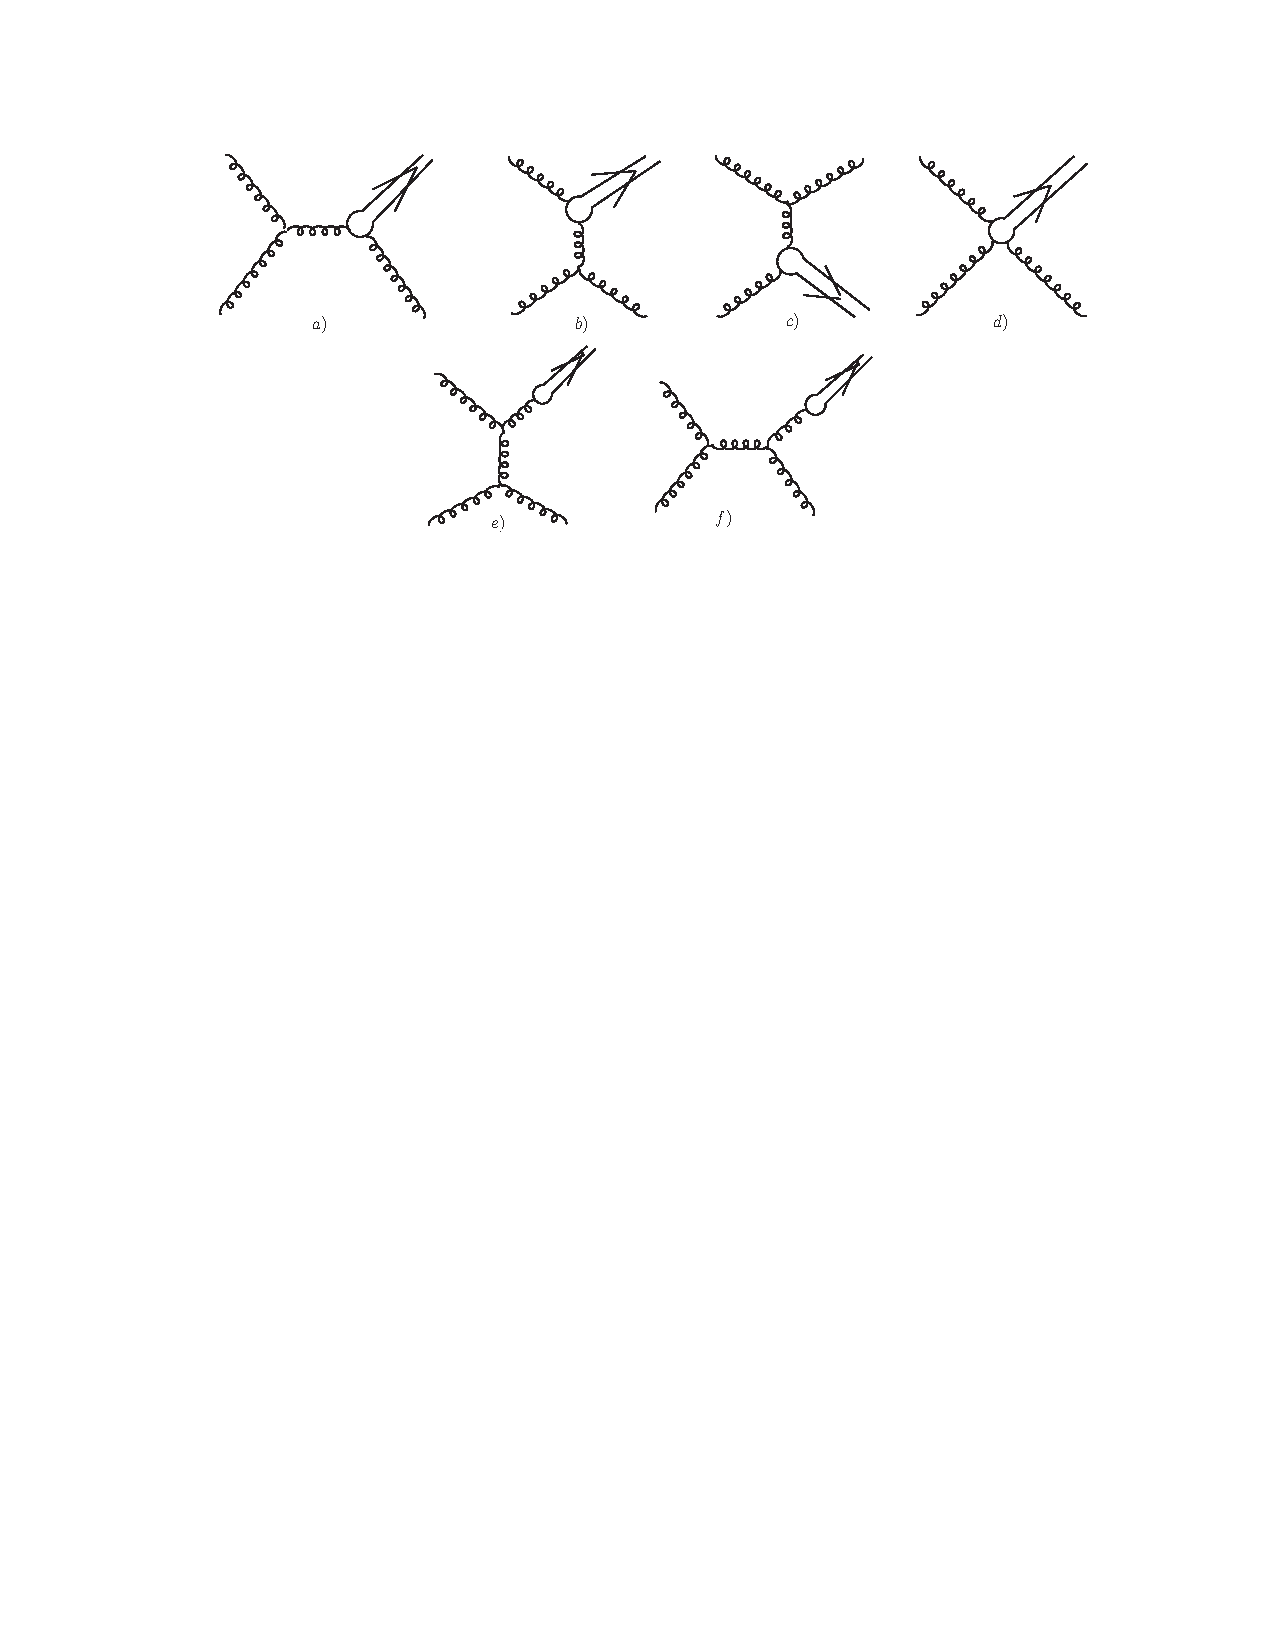
\includegraphics[width=.75\textwidth]{figs/review/chibprod_fig1}
\caption{From Ref.~\cite{Likhoded:2012hw}: Feynman diagrams of the $gg\rightarrow \chi_b g$ NLO 
process. The diagrams in the top row give both CS and CO contributions, the ones in the 
bottom row result only in CO contributions.}
\label{fig:chibprod_fig1} 
\end{figure} 

In this way, all three P-wave states can be produced. The color singlet model
can accommodate the observed $p_T$ dependence of production cross-section.
However, the absolute normalization is several time smaller than measured. This
discrepancy can be solved for the $\chi_c$ spectrum (see \Cref{fig:chibprod_fig2})
by considering color-octet contributions.

\begin{figure}
\center
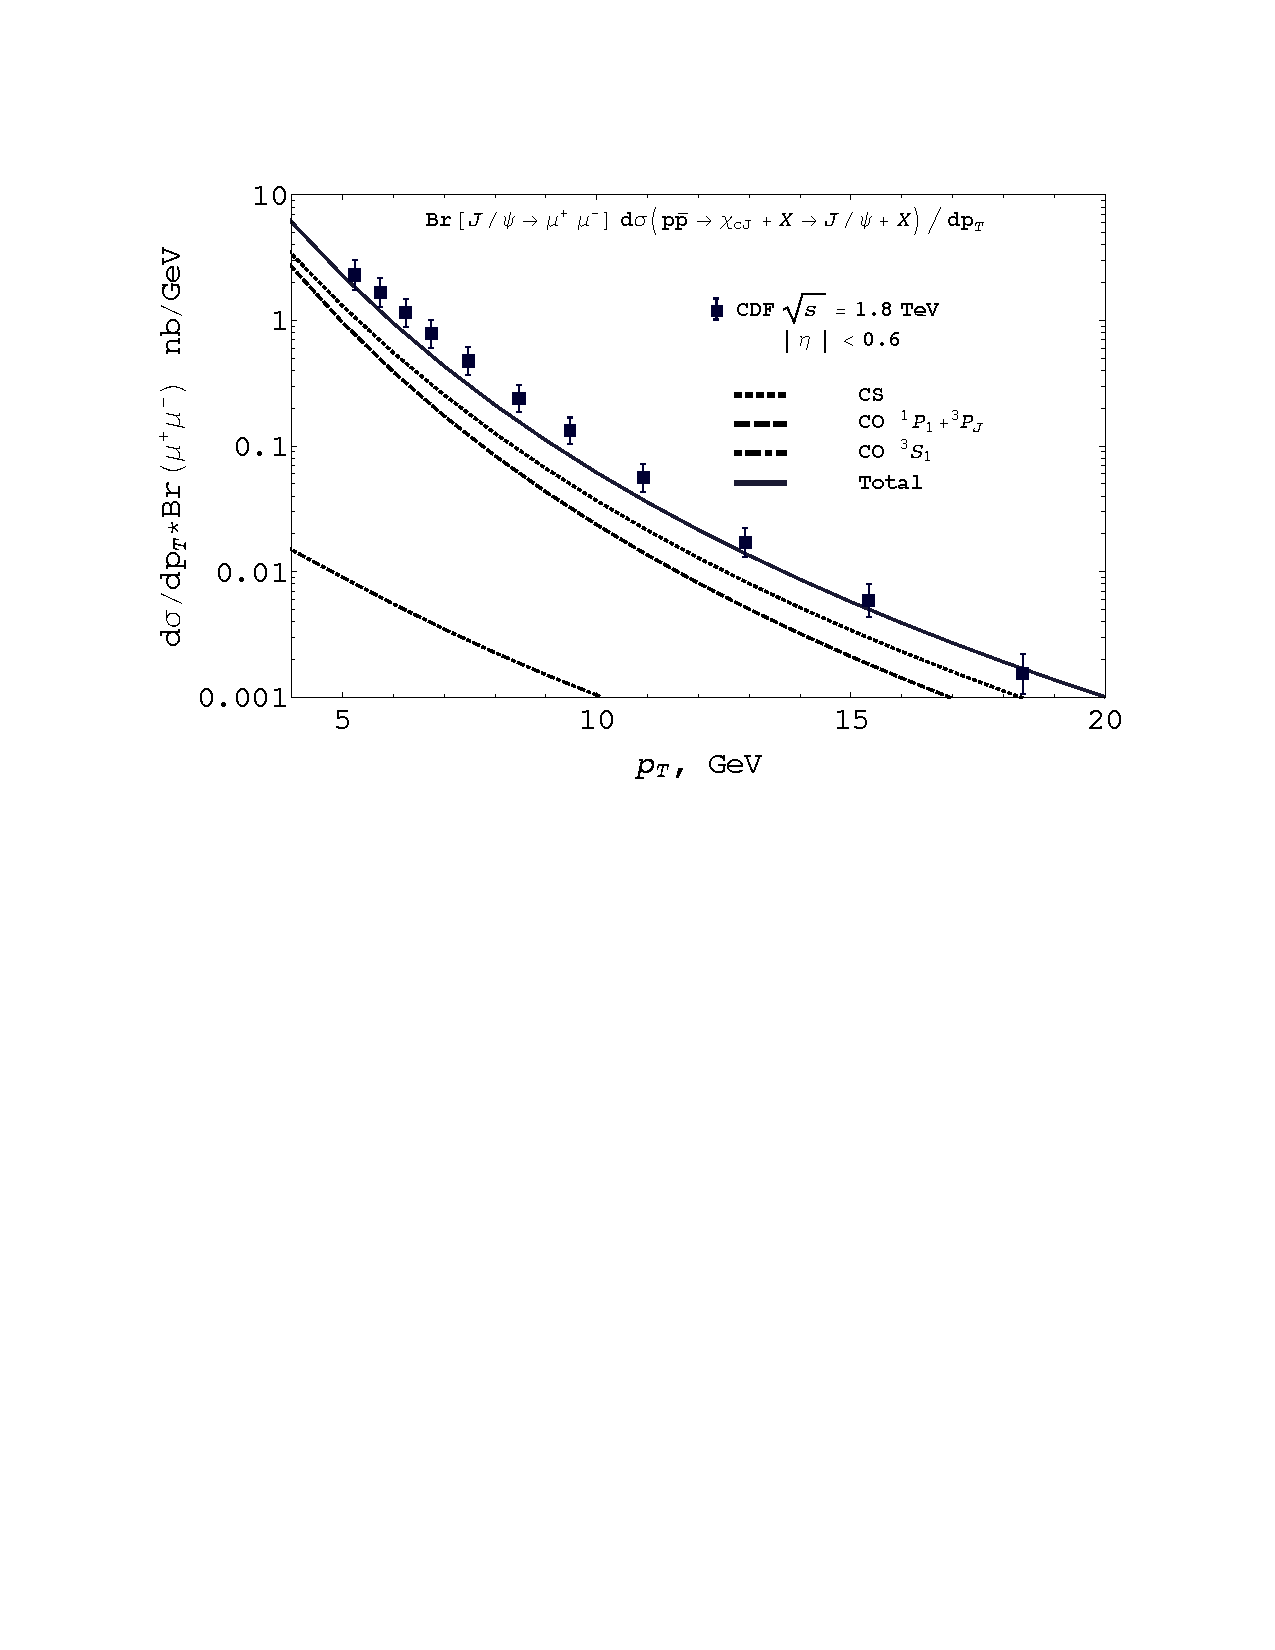
\includegraphics[width=.75\textwidth]{figs/review/chibprod_fig2}
\caption{From ~\cite{Likhoded:2012hw}: Differential production cross section for $\chi_c$ mesons, 
as a function of $p_T$. The different lines correspond to CS (dotted), two different CO 
contributions (dashed and dot-dashed), total (solid). Experimental points are taken from a 
CDF report~\cite{Abulencia:2007bra}.}
\label{fig:chibprod_fig2} 
\end{figure} 

Moreover, predictions for the production cross sections of $\chi_b$ states are
given (see \Cref{fig:chibprod_fig3}).

\begin{figure}
\center
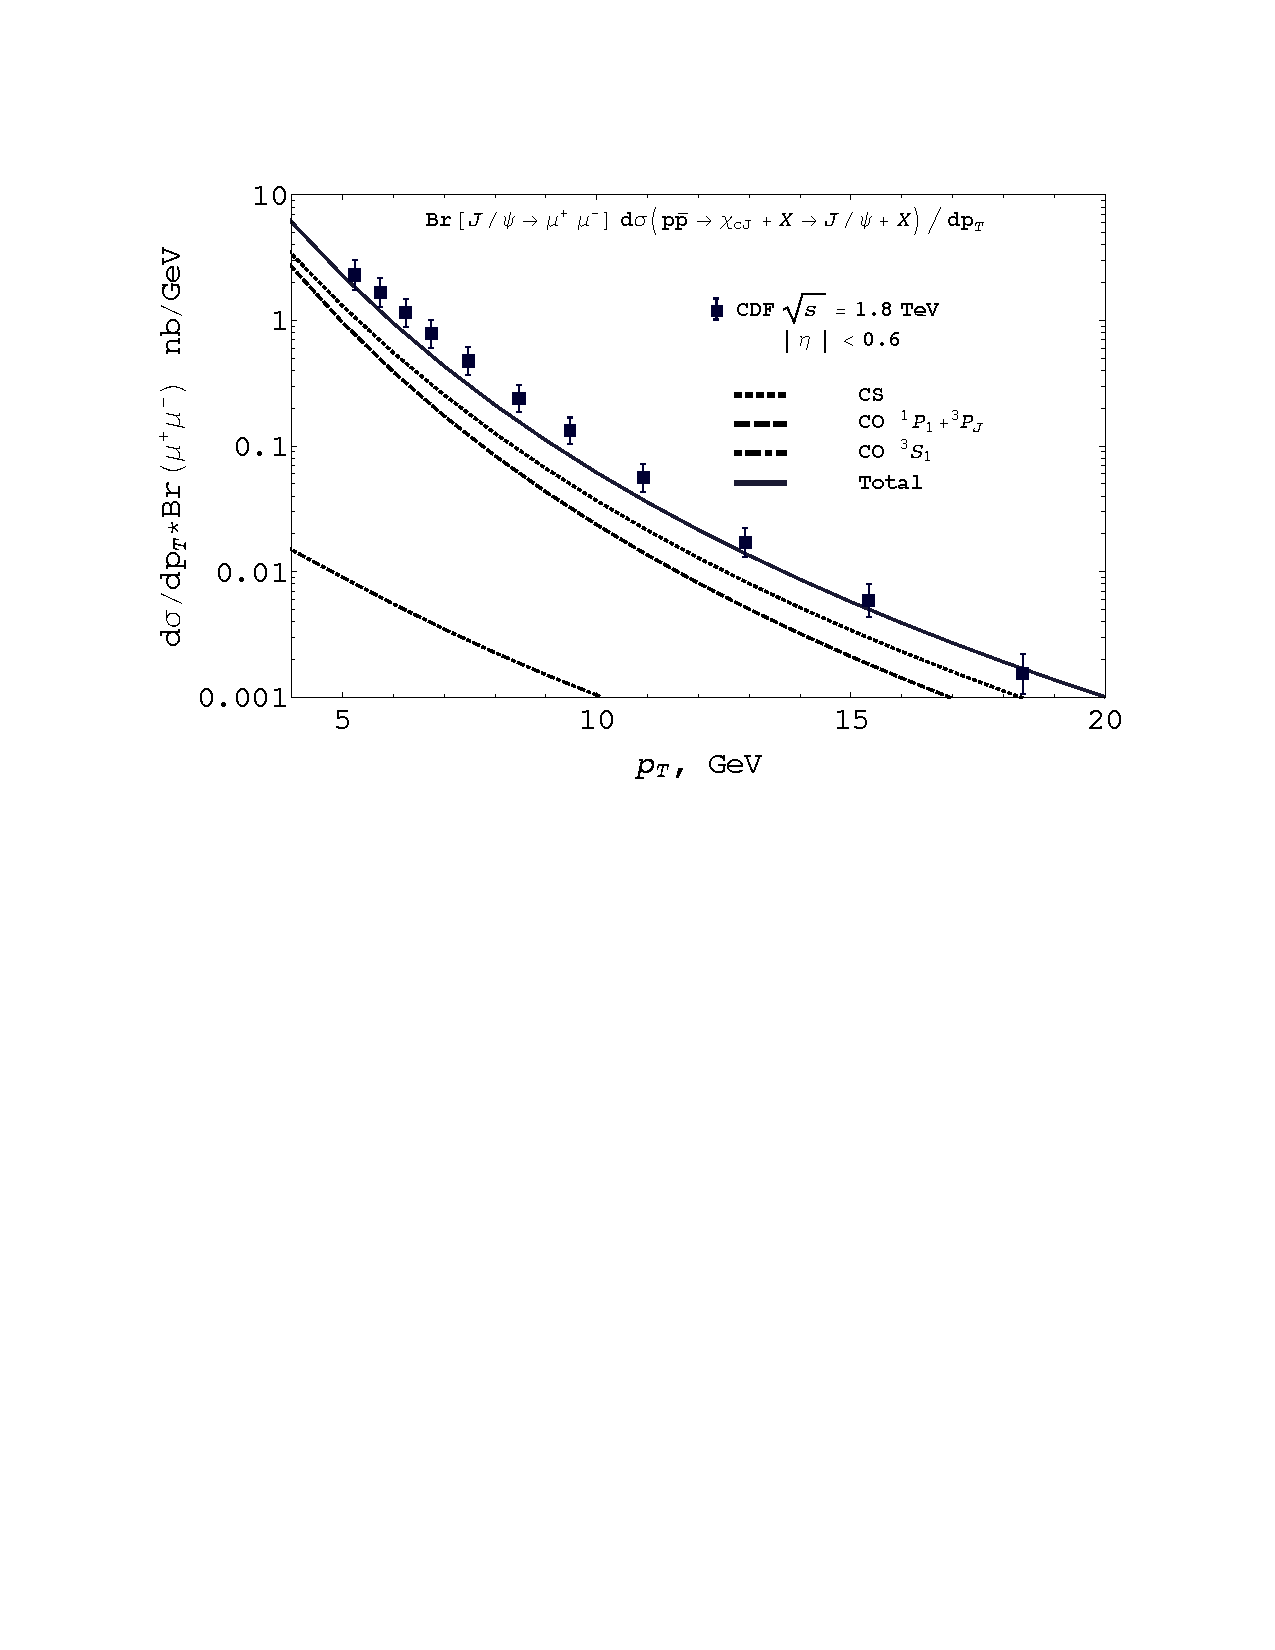
\includegraphics[width=.75\textwidth]{figs/review/chibprod_fig3}
\caption{From Ref.~\cite{Likhoded:2012hw}: Transverse momentum distribution for $\chi_b$ states at 
$\sqs=8\tev$.}
\label{fig:chibprod_fig3} 
\end{figure} 

Also, the ratio between different spin states as a function of transverse
momentum gives a good description of $\chi_c$ data and can be used to infer the
corresponding ratio for $chi_b$ states, see \Cref{fig:frac:ratio}.

\begin{figure}[ht]
  \setlength{\unitlength}{1mm}
  \centering
  \resizebox{.75\textwidth}{!}{
  \begin{picture}(75,60)
    %
     \put(0,0){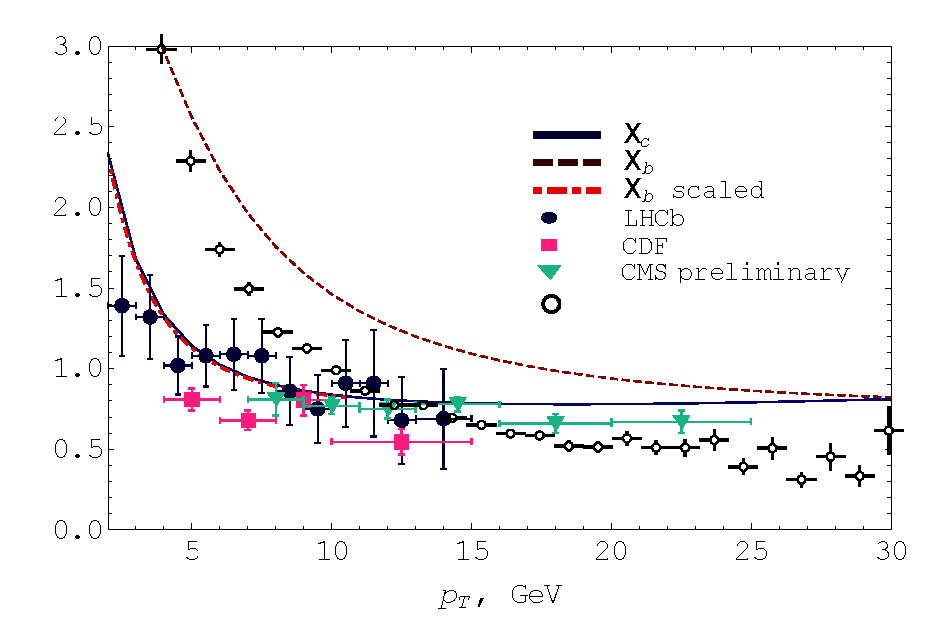
\includegraphics[width=75mm, height=60mm]{ratio/theory}}
     \put(-1,22){\begin{sideways}$\sigma({\chi_2})/\sigma({\chi_1}$)\end{sideways}}
   \end{picture}
  }
  \caption {\small This figure is taken from~\cite{Likhoded:2012hw} and shows
  transverse momentum distributions of the
$d\sigma\left[\chi_{2}\right]/d\sigma[\chi_{1}]$ ratio. Solid and dashed lines
stand for charmonium and bottomonium mesons. The dot-dashed line corresponds to
the rescaled bottomonium ratio:
$\sigma_{b2}/\sigma_{b1}(M_{\chi_c}/M_{\chi_b}p_T)$. The experimental results
for charmonium from LHCb\cite{LHCb-PAPER-2013-028} are shown with dots,
CDF~\cite{Abulencia:2007bra} --- with rectangles, and CMS~\cite{Chatrchyan:2012ub}
--- with triangles.}
  \label{fig:frac:ratio}
\end{figure} 
